%%%%%%%%%%%%%%%%%%%%%%%%%%%%%%%%%%%%%%%%%%%%%%%%%%%%%%%%%%%%%%%%%%%%%%%%%%%%%%%%%%%%%%%%%%%%%%%%%%%%%%%%%%%%%%%%%%%%%%%%%
\subsection{Motivation}
%%%%%%%%%%%%%%%%%%%%%%%%%%%%%%%%%%%%%%%%%%%%%%%%%%%%%%%%%%%%%%%%%%%%%%%%%%%%%%%%%%%%%%%%%%%%%%%%%%%%%%%%%%%%%%%%%%%%%%%%%

%%%%%%%%%%%%%%%%%%%%%%%%%%%%%%%%%%%%%%%%%%%%%%%%%%%%%%%%%%%%%%%%%%%%%%%%%%%%%%%%%%%%%%%%%%%%%%%%%%%%%%%%%%%%%%%%%%%%%%%%%
\begin{frame}
\frametitle{Sensor Calibration}

\begin{columns}
\column{0.5\textwidth}
% With the development of more complex robotic and intelligent systems, many now contain \textbf{several sensors, often of multiple modalities}

% \pause
\begin{block}{}
Multi-sensor or multi-modal perceptual systems operate under the assumption that accurate geometrical
transformations between the sensors that collect the data are known
\end{block}

\column{0.5\textwidth}
\begin{center}
\begin{tabular}{c}
\onslide<1->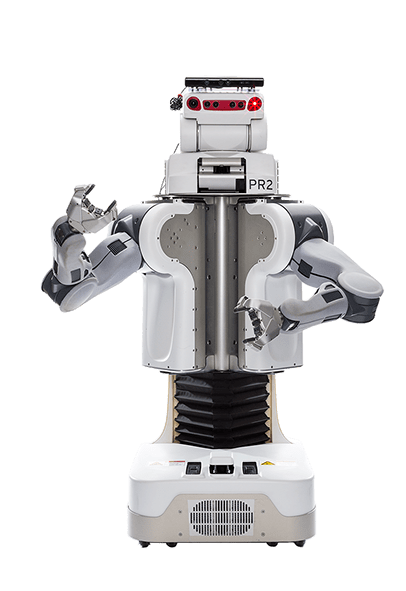
\includegraphics[width=0.8\textwidth]{img/pr2/pr2_a}
% 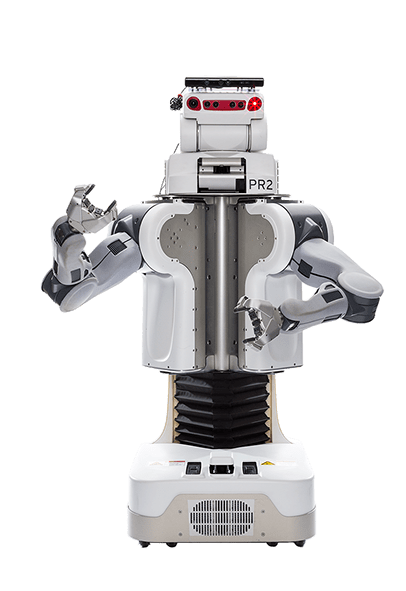
\includegraphics[width=0.8\textwidth]{img/pr2/pr2_a}
\end{tabular}
\end{center}
\end{columns}
\end{frame}
%%%%%%%%%%%%%%%%%%%%%%%%%%%%%%%%%%%%%%%%%%%%%%%%%%%%%%%%%%%%%%%%%%%%%%%%%%%%%%%%%%%%%%%%%%%%%%%%%%%%%%%%%%%%%%%%%%%%%%%%
\begin{frame}
\frametitle{ATOM Calibration Framework}
\begin{columns}
\column{0.5\textwidth}

\begin{itemize}
    \item A general sensor calibration framework
    \item Based on an optimization algorithm
    \item Potential for enhancement
\end{itemize}

\column{0.5\textwidth}
\end{columns}
\end{frame}
%%%%%%%%%%%%%%%%%%%%%%%%%%%%%%%%%%%%%%%%%%%%%%%%%%%%%%%%%%%%%%%%%%%%%%%%%%%%%%%%%%%%%%%%%%%%%%%%%%%%%%%%%%%%%%%%%%%%%%%%